\chapter{Effect of measurement uncertainty}
\label{cha:error}
% **************************** Define Graphics Path **************************
\ifpdf
    \graphicspath{{Chapter4/Figs/Raster/}{Chapter4/Figs/PDF/}{Chapter4/Figs/}}
\else
    \graphicspath{{Chapter4/Figs/Vector/}{Chapter4/Figs/}}
\fi

% **************************** Chapter Abstract ******************************
\leftskip=1cm
\noindent
\emph{Observations are inevitably contaminated with measurement uncertainty, which is a predominant source of uncertainty in some cases. In reliability analysis, probabilistic models are typically fitted to measurements without considering this uncertainty. Hence, this chapter intends to explore the effect of this simplification on structural reliability and to provide recommendations on its treatment. Statistical and interval-based approaches are used to quantify and to propagate measurement uncertainty. They are critically compared by analyzing ground snow measurements, which are often affected by large measurement uncertainty. It is propagated through the mechanical model of a generic structure to investigate its effect on reliability. 
%Parametric studies facilitate to analyze the effect of key parameters, such as measurement uncertainty, coefficient of variation of ground snow load, and distribution type. The interval analysis is performed as a hybrid interval-probabilistic analysis. Measurements are represented as intervals and probabilistic model is then fitted to them. Thus, snow parameters and the reliability index are also interval variables; other random variables are described by standard probabilistic distributions. Implementation of the statistical approach is based on the frequentist paradigm where the contamination mechanism is expressed in terms of random variables. This approach allows decoupling measurement uncertainty from a variable of interest.
The results indicate that measurement uncertainty may lead to significant (order of magnitude) underestimation of failure probability and should be taken into account in reliability analysis. 
%If more information than interval endpoints is available, a statistical approach is recommended; otherwise the interval representation should be used.
Ranges of the key parameters are identified where measurement uncertainty should be considered. For practical applications, the lower interval bound and predictive reliability index are recommended as point estimates using interval and statistical analysis, respectively. The point estimates should be accompanied by uncertainty intervals, which convey valuable information about the credibility of results. 
%Although general recommendations are given, treatment of measurement uncertainty should be handled on a case-specific basis.
}

\leftskip=0pt\rightskip=0pt

%****************************************************************************************
%****************************************************************************************
\section{Problem statement and the state of the art}

Models accounting for all uncertainties are of a considerable interest in structural reliability since these are the bases of design specifications, hence impacting the building and structure stocks of large regions. Snow is particularly important for light-weight structures for which it is typically the governing action. To our knowledge, the effect of snow measurement uncertainty on structural reliability has not yet been studied and other probabilistic models are treated similarly in civil engineering. For instance, neither the joint European research on snow actions \citep{Sanpaolesi1998} or the JCSS Probabilistic Model Code \citep{JCSS_basis} provides any information on the treatment of measurement uncertainty and its effect. Therefore, the aim of this chapter is to explore the effect of this simplification on structural reliability and to provide recommendations on its treatment.

Observations are inevitably contaminated with measurement uncertainty (MU), which is a predominant source of uncertainty in some cases. Uncertainty is understood here as the lack of knowledge (epistemic) and natural variability (aleatory)\footnote{This division is subjective as conditioned on the selected ``model universe''.}  not including known systematic error, which are assumed to be adjusted. In reliability analysis, probabilistic models are typically fitted to measurements without considering their uncertainty. This is the case for snow measurements where often only the snow depth is measured and the applied techniques makes the derived loads highly uncertain, for example, the uncertainty range can reach 50\% of the measured depth\footnote{Based on a personal correspondence with a meteorologist.}. 

The World Meteorological Organization conducted a comprehensive comparative study on the then available solid precipitation measurement techniques and experimentally confirmed that measurements should be adjusted for wetting loss, evaporation loss, and wind induced undercatch \citep{Goodison1998}. They found that the snow catch ratio of the four most widely used gauges ranges from 20\% to 70\% at 6 m/s wind speed. Even for automated systems, measurement error in solid precipitation can vary from 20\% to 50\% due to undercatch in windy conditions \citep{Rasmussen2012}. Although these mainly contribute to systematic error they indicate uncertainties in snow measurements as these errors cannot be exactly corrected. For instance coefficient of determination ($R^2$) values vary from 0.40 to 0.80 for the fitted wind correction equations at certain sites; these are associated with about 10\% standard error in catchment ratio. Additional uncertainty may be introduced if no site specific auxiliary data, e.g. wind speed measurements, are available \citep{Goodison1998}. These issues are not limited to snow measurements but valid for all evidence based models -- that is for every model -- although their importance may vary.

%****************************************************************************************
%****************************************************************************************
\section{Solution strategy}
%*****************************************************************************************
\subsection{Adopted approaches}

We assume that measurements are corrected for known systematic errors. Additionally, the following model is assumed to describe the connection between observed ($Y$) and real, true, physical ($X$) values, i.e. the variable of interest:
\begin{equation}
\label{eq:ro_link}
	\mathrm{(true, real\footnotemark)} X \xrightarrow[]{h(X,E)} Y \mathrm{(observed)}.
\end{equation}
\footnotetext{Herein we tacitly assume the existence of some objective reality independent of the observer.}
The $h(X, E)$ function represents the mathematical relationship between the true and observed random variables referred hereinafter as reality-observation link. $E$ covers the unknown processes contributing to measurement uncertainty. The recommended probabilistic models -- typically distributions -- in the literature are almost exclusively given for the true variable and not for the observed, potentially contaminated one. Possible reasons for this are that:
\begin{itemize}
	\item The contamination is commonly site- and measuring technique-dependent, thus no general recommendations can be given for the distribution of $Y$.
	\item The model type is often selected based on theoretical arguments considering the physical phenomena generating $X$, for example Normal distribution if $X$ is the result of summation; Lognormal if $X$ is the product of random variables; extreme value distribution if $X$ is related to extremes.
	\item Structural reliability ultimately depends on $X$ and not on $Y$, although we are limited to access only $Y$.
\end{itemize}

The last point is especially important since structures are subjected to actions coming from $X$ and not from $Y$; the latter is affected by our ignorance or inability to make accurate measurements (epistemic uncertainty). In a broader sense this also applies for $X$, but for now we remain in the commonly accepted model universe of engineering and treat $X$ as a random variable. If the distribution type of $X$ is known or agreed, then the reality-observation link uniquely determines the distribution of $Y$. Hence, if any measurement uncertainty is present, its distribution type almost certainly differs from the distribution of $X$. This is prevalently neglected while fitting distributions in civil engineering -- $Y$ is assumed to be distributed as $X$. This simplification is acceptable in some practical cases. This method is termed hereinafter as Approach~1 while it is referred to as Approach~2 when the difference between distributions is appreciated:
\begin{description}
	\item[Approach~1] Use the probabilistic model of true random variable ($X$) and treat the observations -- contaminated with measurement uncertainty -- ($\mathbf{y}$) as the realizations of this model: $\mathbf{y} \sim X$.
	\item[Approach~2] Differentiate between the distribution of true and observed random variables. Within this, the following two sub-approaches are considered:
	\begin{description}
		\item[Approach~2a] Representation of measurement uncertainty with intervals at the level of observations and propagating them to the derived parameters via interval analysis. As interval representation by nature contains no information about the reality-observation link, the decontamination of observations is not possible.
		\item[Approach~2b] Representation of measurement uncertainty with a probability distribution. Use a mathematical model ($h(X, E)$) to describe the connection between measurement uncertainty ($E$), true phenomenon ($X$), and observed phenomenon ($Y$). Based on this model and on observations ($\mathbf{y}$), infer the parameters of the true random variable ($X$). These issues are referred to as \textit{measurement error problems} in the literature \citep{Kondlo2010}.
	\end{description}
\end{description}

\noindent Additional assumptions for all considered approaches:
\begin{itemize}
	\item ${\mathbf{y}} = \left\{ {{y_1},{y_2},...,{y_n}} \right\}$ and ${\mathbf{x}} = \left\{ {{x_1},{x_2},...,{x_n}} \right\}$ each are independent, identically distributed realizations; $\mathbf{y}$ is contaminated with measurement uncertainty.
	\item The realizations of the true phenomenon ($\mathbf{x}$) and measurement uncertainty ($\boldsymbol{\epsilon}$) are mutually independent.
	\item The true phenomenon ($X$) follows arbitrary, but known distribution type.
	\item Only for Approach~2b: the measurement uncertainty ($E$) follows arbitrary, but known distribution type, and the reality-observation link is also known.
\end{itemize}

%Fig 1

%****************************************************************************************
%****************************************************************************************
\subsection{Uncertainty representation and propagation}
\label{sec:uncertainty_rep_prop}

%*****************************************************************************************
\subsubsection{Interval analysis}

Interval representation is one possible approach to quantify uncertainty in an observed variable: the width of the interval expresses our uncertainty (Figure \ref{fig:obs_with_interval}). In this concept the true value is certainly within the interval but we know nothing about how likely it takes a particular value from that. In other words no probability distribution function is assumed over the interval, thus it expresses greater ignorance than probability distributions can \citep{Huber2010}.
The basic objective of interval analysis is to propagate the interval uncertainty of input variables to the outputs. Its main challenge is to calculate the interval bounds without overestimating them. This typically occurs if floating point computations are simply replaced by intervals and caused by interval dependency \citep{Moore2009}. Since the operators are typically not known explicitly and are non-monotonic, special algorithms are needed to obtain sufficiently narrow approximate interval bounds.
Interval analysis is traditionally used to model floating point truncation error in numerical computations; however, it is also successfully applied to various civil engineering issues, for instance, reliability of structures \citep{Qiu2008} and systems \citep{Qiu2007}. \citet{Rao2015} analyzed the effect of incorrect fitting on trusses and frames using mixed interval finite element formulation, using intervals to model fabrication errors. \citet{Muhanna2015} demonstrated the feasibility of non-linear interval finite element analysis for beam-column structures. In their study geometric, material and load uncertainties are modeled with intervals.
In this study the general definition of interval variables is used and constrained numerical optimization is applied to find the interval endpoints. This is motivated by the readily available optimization algorithms, and its feasibility due to the analyzed simple, computationally cheap examples. For computationally demanding models more efficient algorithms are available \citep{Zhang2010, Alibrandi2015, Muhanna2015}.
Intervals in this study are defined by midpoint and radius ($\epsilon_\mathrm{r}$), the midpoint is taken as the observed value, $y_i$, see Figure \ref{fig:obs_with_interval}. In this approach, the true value is assumed to be certainly within the interval given the modeling assumptions are valid.
\begin{figure}[htbp!] 
	\centering    
	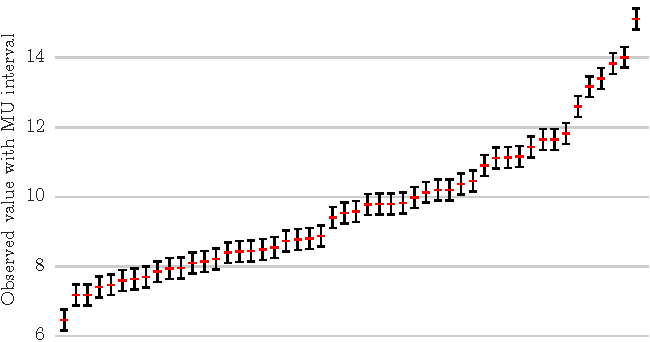
\includegraphics[]{obs_with_interval.pdf}
	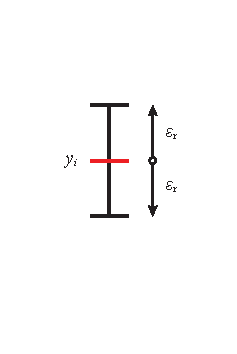
\includegraphics[]{MU_interval.pdf}
	\caption{Interval representation of measurement uncertainty (black) on a sorted random sample (red). The sample is generated from $Q_1$ with properties given in Table \ref{tab:prob_models_mu} and $CV_{Q_1} = 0.2$.}
	\label{fig:obs_with_interval}
\end{figure}

%*****************************************************************************************
\subsubsection{Statistical analysis}
An alternative approach to represent measurement uncertainty is statistical by means of probability distributions. The likelihood function depends on the reality-observation link (Eq.\ref{eq:ro_link}). This connection is also uncertain, but for simplicity, known relationship is assumed here and a possible treatment of this uncertainty is discussed in Section \ref{sec:discussion_mu}. Algebra of random variables can be used to obtain the likelihood function reflecting the distribution of involved random variables and the reality-observation link:
\begin{equation}
\label{eq:mu_like}
	L\left( {{{\boldsymbol{\theta }}_X},{{\boldsymbol{\theta }}_E}|{\mathbf{x}},{\boldsymbol{\epsilon }}} \right) = \prod\limits_{i = 1}^n {p\left( {h({x_i},{\epsilon _i})|{{\boldsymbol{\theta }}_X},{{\boldsymbol{\theta }}_E}} \right)}
\end{equation}
where ${\boldsymbol{\theta }}_X$ and ${\boldsymbol{\theta }}_E$ are the parameters of true and measurement uncertainty random variables, respectively.
In Approach~1, this means no additional complication because the observations are assumed to be distributed as the true random variable since the reality-observation link is neglected. However, in Approach~2b the likelihood function should be constructed to remove the effect of measurement uncertainty ($E$) from the variable of interest ($X$).
The \textit{measurement error problem} arises in many areas where only the contaminated values are attainable to the observer but the interest lays in the inference of true, uncontaminated values. Among others, these areas include astronomy, econometrics, biometrics, medical statistics, and image reconstruction \citep{Stefanski2000, Koen2009, Meister2009}. A straightforward solution is to construct the likelihood function (Eq.\ref{eq:mu_like}) and to infer the parameters of the variable of interest ($X$) by a selected method. To our knowledge this approach has not been applied in civil engineering yet.
Maximum likelihood method is used herein to infer the parameters in the statistical formulation of the measurement uncertainty problem.
Additive and multiplicative reality-observation links are considered. For the additive relationship: $Y = X + E$, the density function of the sum of two independent, continuous random variables is obtained by convolution:
\begin{equation}
\label{eq:conv}
	{f_Y}\left( y \right) = \left( {{f_X} * {f_E}} \right)\left( y \right) = \int\limits_{ - \infty }^\infty  {{f_X}\left( {y - x} \right)}  \cdot {f_E}\left( x \right) \cdot {\mathrm{d}}x.
\end{equation}
Here, for convenience the $p(.)$ notation of density functions is replaced with one that identifies the function elsewhere than in the argument, $f_X(x) \equiv p(x)$.
The integral can be efficiently solved by utilizing Fourier transformation since afterwards it reduces to a point-wise multiplication. Here, the fast-Fourier transformation is used to accomplish this task. For the multiplicative relationship: $Y = X \cdot E$, the density function of the product of two independent, continuous random variables is obtained by computing the following integral:
\begin{equation}
\label{eq:prod}
	{f_Y}\left( y \right) = \int\limits_{ - \infty }^\infty  {{f_X}\left( x \right)}  \cdot {f_E}\left( {\frac{y}{x}} \right) \cdot \frac{1}{{\left| x \right|}} \cdot {\mathrm{d}}x.
\end{equation}
This can be efficiently solved by Mellin transformation but here the integral is directly calculated due to the small computational burden.
Sampling variability (parameter estimation uncertainty) is accounted for by using the predictive reliability index, $\tilde \beta$ \citep{Kiureghian1989}:
\begin{equation}
\label{eq:predi_beta}
	 \tilde \beta  = \frac{{{{\mathrm{mean}}_B}}}{{\sqrt {1 + {{\mathrm{std}}_B}^2} }} \approx \frac{{{\mathrm{median}_B}}}{{\sqrt {1 + {{\left( {1.483 \cdot {{\mathrm{mad}}_B}} \right)}^2}} }}
\end{equation}
where $B$ is the posterior reliability index, std and mad are the standard deviation and median absolute deviation of $B$, respectively. The formulation with median and mad are used in this chapter, as that is more robust to outliers. Eq.\ref{eq:predi_beta} is an approximation as it is valid only for Normal distributed $B$. Additionally, the statistics are estimated from repeated analyses, and no Bayesian formulation of the reliability problem is used, even though that was used to derive the formula. For this study it is deemed sufficiently accurate to indicate tendencies and to identify critical cases.
\begin{figure}[htbp!] 
	\centering    
	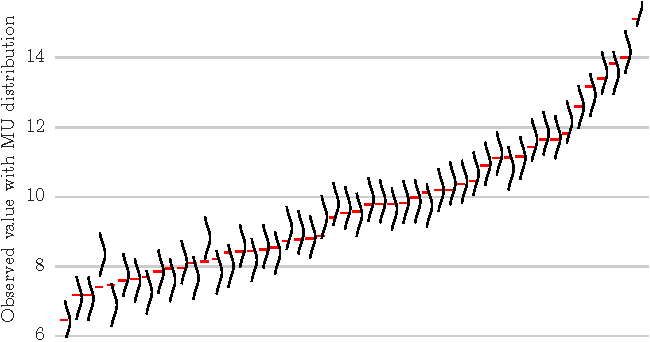
\includegraphics[]{obs_with_prob_error.pdf}
	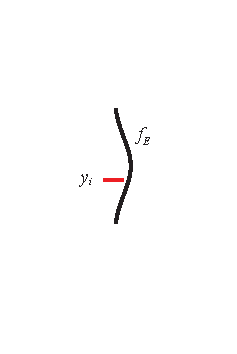
\includegraphics[]{MU_prob_distr.pdf}
	\caption{Illustration of probability distribution representation of measurement uncertainty (black) on a sorted random sample (red). The sample is generated from $Q_1$ with properties given in Table \ref{tab:prob_models_mu} and $CV_{Q_1} = 0.2$.}
	\label{fig:obs_with_prob_error}
\end{figure}

%****************************************************************************************
%****************************************************************************************
\section{Example: reliability of a generic structure}

%*****************************************************************************************
\subsection{Model description}
The reliability of a simple structural member is analyzed using a generic limit state function:
\begin{equation}
	 g(\mathbf{X}) = R - \left( {G + {Q_{50}}} \right).
	 %({\mathbf{X}})
\end{equation}

It represents a structure subjected to permanent ($G$) and variable ($Q_{50}$) actions, where the subscript 50 indicates 50-year reference period (common design working life). The probabilistic model of involved random variables are based on the recommendations of \citep{JCSS_basis} and summarized in Table \ref{tab:prob_models_mu}. For simplicity only the variable action is assumed to be affected by measurement uncertainty; it could be easily extended to more variables. Coefficient of variations 0.2, 0.4 for $Q_1$ represent annual snow maxima of mountains, highlands, while 0.6 characterizes lowlands in the Carpathian Region. The Lognormal model for snow maxima is typically adopted in the USA \citep{ASCE2010}, while the Gumbel model is widespread in Europe \citep{Sanpaolesi1998, JCSS_load}. The Normal and Gumbel distributions are light-tailed while the Lognormal is heavy-tailed. The adopted distributions and parameter ranges cover also other variable actions such as wind and thermal actions, thus the results can be readily generalized.

The annual maxima are assumed to be independent:
\begin{equation}
\label{eq:gfun_mu}
	{F_{50}}\left( q \right) = {F_1}{\left( q \right)^{50}}
\end{equation}
where $F(.)$ is the cumulative distribution function.

\begin{table}[htbp!]
\caption{Probabilistic models.}
\centering
\label{tab:prob_models_mu}
\small
	\begin{threeparttable}
    \begin{tabular}{llll}
    \toprule
    Variable name (symbol)  & Distribution & Mean & CV \\
    \midrule
    \rowcolor{lightgrey} Resistance ($R$)  & Lognormal & \tnote{*} & 0.10  \\
    Permanent action ($G$) & Normal &  8  & 0.10 \\
    \rowcolor{lightgrey} Variable action ($Q_1$)\tnote{\textdagger}  & Normal, Lognormal, Gumbel & 10 & $[0.20, 0.40, 0.60]$ \\
    \bottomrule
    \end{tabular}
    \begin{tablenotes}
    	\item[*] set to reach $\beta_\mathrm{target} = 3.8$ for each combination of inputs.
	    \item[\textdagger] the specified parameters are used to generate 50-element sample and the parameters of the model used in reliability analysis are inferred from it.  
   	\end{tablenotes}
   	\end{threeparttable}
\end{table}

\subsection{Interval and reliability analysis}
\label{subsec:interval_reli}
To model the effect of measurement uncertainty, 50 random observations are generated from $Q_1$, these are treated as observed ($Y$) values as the reality-observation link by definition is unknown in interval representation (Figure \ref{fig:int_alg}). Then intervals are centered at observations and various interval radiuses are considered. Using these interval variables, the distribution of $Q_1$ is fitted by the method of moments, which is a widely used approach in civil engineering \citep{Sanpaolesi1998} and was proved to be robust e.g. for modeling hydrological extremes \citep{Madsen1997}. The hybrid interval-probabilistic reliability problem is solved using optimization and first order reliability method (FORM). An outcome of the analysis is an interval reliability index.

The upper bound of it is irrelevant from safety point of view and the lower bound is recommended for practical applications \citep{Qiu2007}. This is due to the special nature of intervals and how they represent uncertainty: the real value can be anything within the interval but one cannot assume that all points are equally likely (principle of indifference) at least because the consequence of specific values are not equal. Hence we chose the recommended, careful engineering approach and use the lower endpoint of the reliability index interval as representative value.
\begin{figure}[htbp!] 
	\centering    
	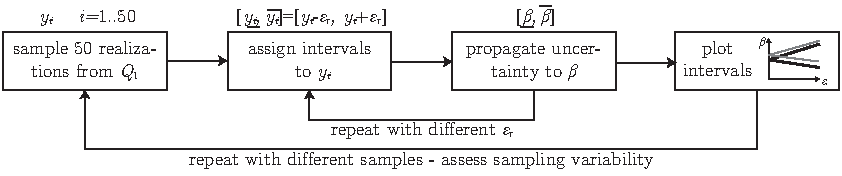
\includegraphics[]{interval_analysis_algorithm_.pdf}
	\caption{Algorithm of analyzing the effect of interval measurement uncertainty on reliability.}
	\label{fig:int_alg}
\end{figure}

\subsubsection{Full and approximate propagation of interval uncertainty}
As measurement uncertainty is expressed at the level of individual observations its full propagation yields to two distinct 50-dimensional constrained optimization problems that can be computationally demanding if each iteration step involves fitting a distribution function and solving a reliability problem. The computational burden can be considerably lessened by a two-step approximate technique where first the distribution parameters are fitted to the interval observations. Then only the interval representation of distribution parameters are used in further reliability analysis. Thus, the optimization with reliability analysis is reduced to a two-dimensional search space. Moreover, our experience show that the optimum is at the bounds so as it can be found by considering only the possible permutations of the parameter bounds.
The accuracy of full and two-step approximate uncertainty propagations are compared using Gumbel distributed $Q_1$. The results in terms of reliability indices are presented in Figure \ref{fig:beta_interval_full_approx}. The interval uncertainty is expressed as the ratio of interval radius and mean of annual maxima ($Q_1$). 0-10\% range is covered and it is assumed that all observations are contaminated with the same radius. For each coefficient of variation the mean of the resistance is set to reach the 3.8 target reliability level. This is performed by considering no measurement uncertainty ($\epsilon_\mathrm{r} = 0$) and using the parameters given in Table \ref{tab:prob_models_mu}, thus sampling variability has no effect. The calculated upper and lower reliability index endpoints are presented in the plots with solid and dashed lines for two-step and full propagations, respectively. Figure \ref{fig:beta_interval_full_approx} shows also the reliability index obtained by Approach~1. This is illustrated with a dotted line and is not affected by the assumed measurement uncertainty interval.
\begin{figure}[htbp!] 
	\centering    
	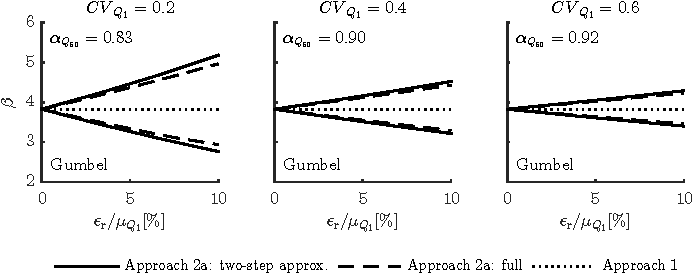
\includegraphics[]{beta_interval_full_approx.pdf}
	\caption{Reliability index intervals as the function of normalized measurement uncertainty radius ($\epsilon_\mathrm{r}/\mu_{Q_1}$) with full and approximate propagation of interval uncertainty.}
	\label{fig:beta_interval_full_approx}
\end{figure}

The plots show that the approximate technique slightly overestimates the accurate (full) reliability intervals, the largest difference is observed for $CV_{Q_1} = 0.2$ with large measurement uncertainty. Since in general the overestimation of the approximate technique is small, it is used in all further analysis. The sensitivity factor of the 50-year reference period maxima ($\alpha_{Q_{50}}$) is also displayed on the plots. It corresponds to a model without uncertainty in measurement and parameters. The decreasing interval range of $\beta$ with increasing $CV_\mathrm{Q1}$ is explained by the decreasing contribution of interval uncertainty to the full uncertainty of $Q_1$, i.e. aleatory uncertainty becomes dominating. Figure \ref{fig:explain_decr_beta_int} illustrates this shrinkage of uncertainty interval by comparing the transformed cumulative distribution functions with different coefficient of variations. The plots correspond to 50 particular random realizations; the same pattern is observed for other sets of random realizations.
\begin{figure}[htbp!] 
	\centering    
	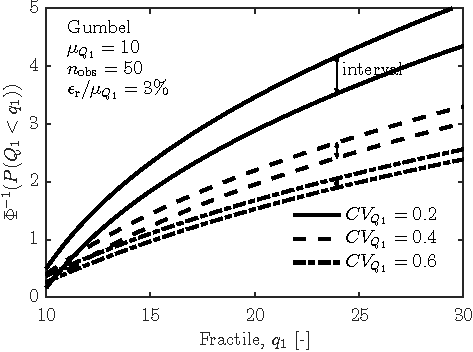
\includegraphics[]{explain_decr_beta_int.pdf}
	\caption{Illustration of the shrinkage of uncertainty interval with increasing coefficient of variation but constant measurement uncertainty interval.}
	\label{fig:explain_decr_beta_int}
\end{figure}

\subsubsection{Effect on reliability index and required resistance}
Eq.\ref{eq:gfun_mu} is solved for Normal, Lognormal and Gumbel distributed variable action ($Q_1$) using the two-step approximation technique. The results are summarized in Figure \ref{fig:beta_interval_small_multiples}; they have the same rationale as is given for Figure \ref{fig:beta_interval_full_approx}. The light gray lines show the opening reliability interval with increasing measurement uncertainty for 20 random samples, each with 50 realizations. These are indicative of the effect of sampling variability: in this case this is entirely parameter estimation uncertainty due to the finite sample size. The results show that sampling variability -- with 50 realizations, which is typical for maxima model of climatic actions -- has significant effect on reliability. It is dominating over measurement uncertainty for small interval radiuses and comparable for larger values. The thick black lines are the median of the 20 sample sets. The reliability index without considering measurement uncertainty can be seen at the common starting point of the lower and upper bound lines. The difference of this value and the lower bound is of interest here as it indicates the extent of the non-conservative neglect of measurement uncertainty. Based on our experience, the difference is deemed significant if it is larger than 0.5. This level is indicated by a dashed horizontal line while the significant range with a red half line. With the selected target reliability level, this corresponds to more than six-fold increase in failure probability.
\begin{figure}[htbp!] 
	\centering    
	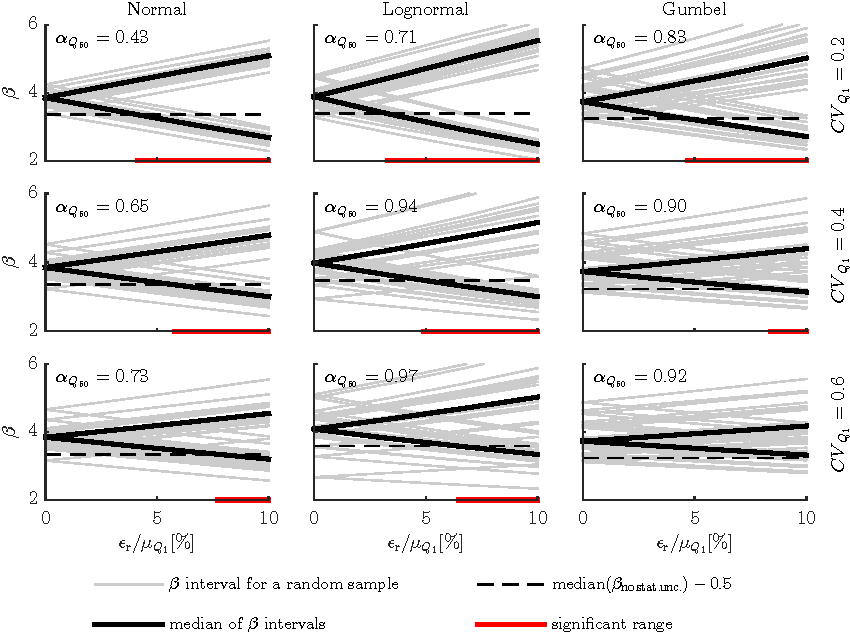
\includegraphics[]{beta_interval_small_multiples.pdf}
	\caption{Reliability index intervals as the function of the normalized measurement uncertainty radius ($\epsilon_\mathrm{r}/\mu_{Q_1}$). The gray lines represent 20 random samples, indicating sampling variability. The black lines are the median lower and upper interval endpoints of the reliability index. The red half line indicates the range where the lower endpoint of the reliability interval is significantly lower ($>0.5$) than the reliability calculated without measurement uncertainty ($\epsilon_\mathrm{r} = 0$).}
	\label{fig:beta_interval_small_multiples}
\end{figure}

The results suggest that moderate $\pm 4\%$ measurement uncertainty can lead to significant reduction of reliability level for mountains and highlands represented by $CV_{Q_1} = 0.2-0.4$. For the largest considered value of $CV_{Q_1} = 0.6$, the Gumbel model does not reach the limiting value. This indicates that for lowlands even a quite large $\pm 10\%$ measurement uncertainty has no practically significant effect. The reliability interval ranges indicate that even a small $\pm 2\%$ measurement uncertainty can lead to an order of magnitude uncertainty in the failure probability, see for instance the Lognormal distribution with $CV_{Q_1} = 0.2$. For larger measurement uncertainties, the width of the reliability intervals can be larger than 2.0; the widths are quite considerable for large $CV_{Q_1} = 0.6$ models too.
Measurement uncertainty thus seems to have a marked effect on structural reliability. The practical question then arises: what are its implications on design and how it should be accounted for? To examine this, we calculated the mean resistance ($\mu_R$) required to reach the target reliability with the lower bound of the reliability interval (Approach~2a). Then this value is compared to the $\mu_R$ required to reach the target reliability without explicit consideration of measurement uncertainty (Approach~1). The ratios of the mean values (with interval MU/without explicit MU) are illustrated in Figure \ref{fig:dspt_ratio_small_multiples}. These indicate how large adjustment might be needed in representative resistance values to meet target reliability in the presence of measurement uncertainty. The plots are structured and have the same rationale as Figure \ref{fig:beta_interval_small_multiples}. Based on our expertise, the ratio is deemed practically significant if it is larger than 1.1. This level is indicated by a dashed horizontal line while the significant range with a red half line. The small effect of sampling variability for Normal distribution is likely due to the small sensitivity factor of $Q_{50}$. On the contrary, sampling variability is quite considerable for Lognormal distribution. The selected threshold is reached for all distributions. The Lognormal model shows opposite trend, this might be attributed to its heavy tail. For this distribution the 1.1 threshold is reached at about 4\% normalized radius and the ratio can be over 1.4 for larger radiuses, which is a huge potential adjustment. The Gumbel distribution illustrates decreasing ratio with increasing coefficient of variation. For $CV_{Q_1} = 0.2$ (mountains), moderate $\pm 4\%$ measurement uncertainty can lead to significant $\mu_R$ ratio. For lowlands ($CV_{Q_1} = 0.6$), the ratio is over the selected threshold only for excessive measurement uncertainty $\pm 9\%$, which suggests that measurement uncertainty can be neglected for large values of $CV_{Q_1}$.
\begin{figure}[htbp!] 
	\centering    
	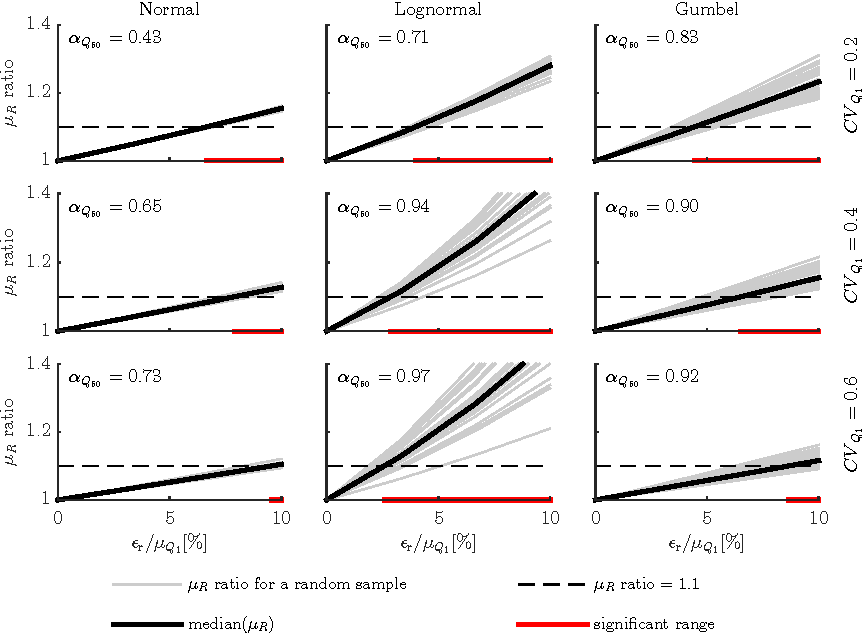
\includegraphics[]{dspt_ratio_small_multiples.pdf}
	\caption{Mean resistance ($\mu_R$) ratio for the variable action with and without measurement uncertainty as the function of the normalized measurement uncertainty radius ($\epsilon_\mathrm{r}/\mu_{Q_1}$). The red half line indicates the significant range where the ratio is larger than 1.1.}
	\label{fig:dspt_ratio_small_multiples}
\end{figure}

\subsection{Statistical and reliability analysis}
This section presents the statistical approach to quantify and propagate measurement uncertainty (Approach~2b). To model the effect of measurement uncertainty, 50 random observations are generated from $Q_1$ and treated as true ($X$) values. Then by using the assumed reality-observation link they are contaminated with measurement uncertainty. This is generated from a known, independent distribution ($E$). The algorithm is outlined in Figure \ref{fig:stat_alg}. Additive and multiplicative reality-observation links are assumed and the measurement uncertainty is taken as normally distributed with zero mean (unbiased). After the contamination of data, the information about the parameters of the underlying generating models -- with the exception of the zero mean of measurement uncertainty -- is disregarded and the maximum likelihood method is applied to decouple true values from measurement uncertainty. Finally, the model of decontaminated observations is used in reliability analysis. The sampling variability is again indicated by 20 samples and taken into account in an approximate manner through the predictive reliability index (Eq.\ref{eq:predi_beta}). The median and mean absolute deviation are calculated.
\begin{figure}[htbp!] 
	\centering    
	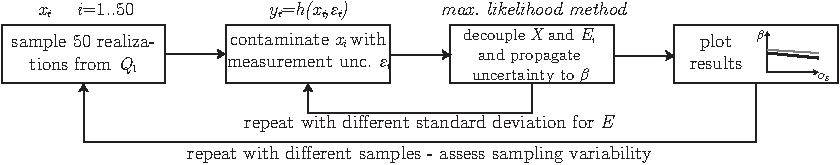
\includegraphics[]{statistical_analysis_algorithm_.pdf}
	\caption{Algorithm of analyzing the effect of measurement uncertainty on reliability using statistical technique.}
	\label{fig:stat_alg}
\end{figure}

\subsubsection{Decontamination of observations}
To illustrate the technique and the effect of decontamination, random realizations are generated from Gumbel distribution -- with parameters given in Table \ref{tab:prob_models_mu} -- and contaminated with measurement uncertainty (Figure \ref{fig:Gumbel_additive_me_smallm}). First, additive reality-observation relationship is assumed and Approach~1 and Approach~2b are used to infer the model parameters. The maximum likelihood method is used to obtain point estimates and the delta method is applied to construct $90\%$ confidence intervals to illustrate parameter estimation uncertainty \citep{Coles2001}.\mynote{ref to chapter 2!} The results for three cases of Gumbel distribution and two cases of measurement uncertainty with varying standard deviation are discussed only. The realizations and the fitted models are shown in Figure \ref{fig:Gumbel_additive_me_smallm}. It comprises return value-return period plots transformed to Gumbel space where the Gumbel distribution appears as a straight line. Though the plots are corresponding to a particular set of realizations, they convey reliably the trends and expected differences: (\textit{i}) Approach~1 typically overestimates the fractiles thus leading to lower reliability level and being conservative; (\textit{ii}) the difference between models increases with increasing return period. Due to the small sample size, the difference is affected by large sampling variability.
The calculations are repeated with multiplicative measurement uncertainty (Figure \ref{fig:Gumbel_prod_me_smallm}). The results correspond well with those obtained for the additive format. Furthermore, wider confidence intervals of Approach~2b compared with Approach~1 are observed. This is due to the larger model space where the same sample size allows less certain inference. This effect is less pronounced for the additive model.
For both models, Approach~1 is inherently biased since it is not using the correct likelihood function, while Approach~2b asymptotically converges to the true model. Thus, in the long run -- from theoretical point of view -- Approach~2b is better; however, Approach~1 seems to be generally conservative for the considered reality-observation links. This latter aspect is analyzed in more detail in the following section focusing on reliability index as a quantity of practical interest.
\begin{figure}[htbp!] 
	\centering    
	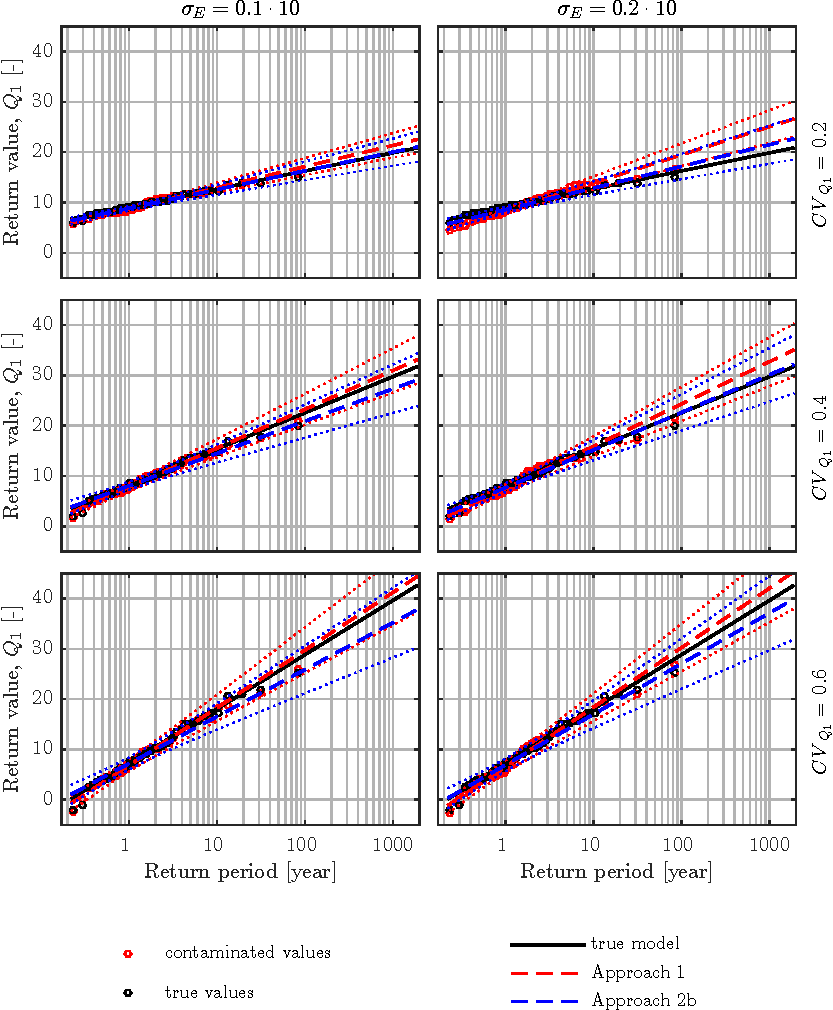
\includegraphics[]{Gumbel_additive_me_smallm_50_rng23.pdf}
	\caption{Gumbel distributions fitted to random realizations contaminated with additive measurement uncertainty using Approach~1 and Approach~2b. The point estimates (dashed lines) are accompanied by 90\% confidence intervals (dotted lines).}
	\label{fig:Gumbel_additive_me_smallm}
\end{figure}
\begin{figure}[htbp!] 
	\centering    
	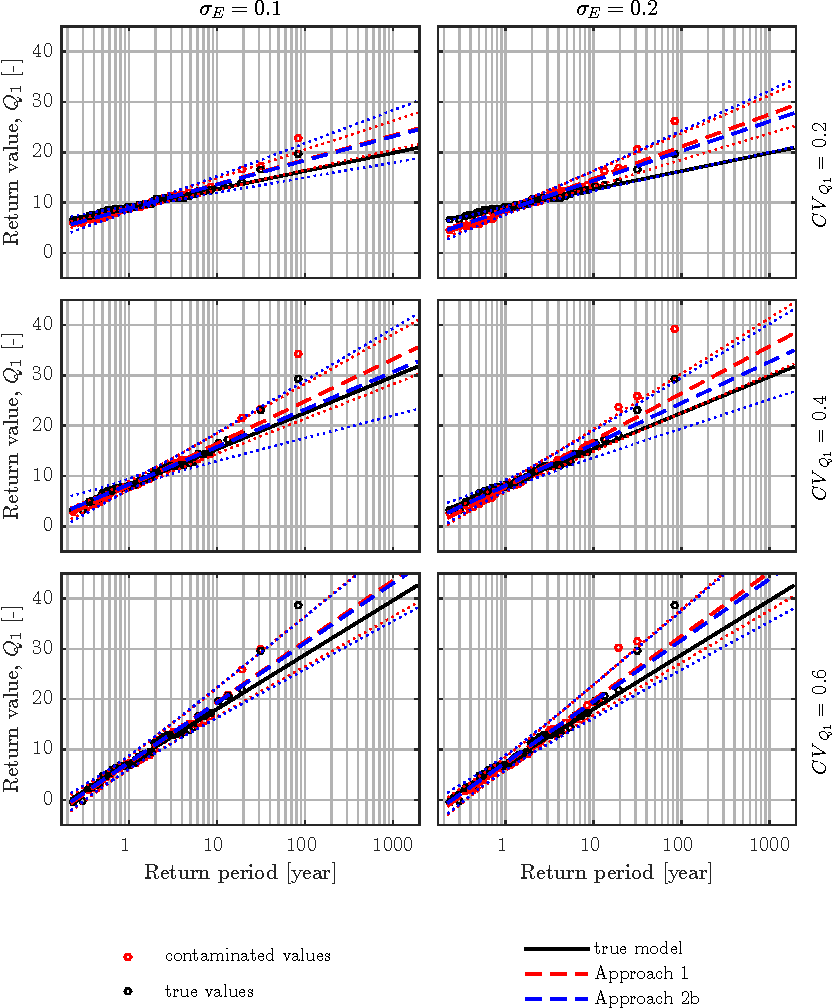
\includegraphics[]{Gumbel_prod_me_smallm_50_rng14.pdf}
	\caption{Gumbel distributions fitted to random realizations contaminated with multiplicative measurement uncertainty using Approach~1 and Approach~2b. The point estimates (dashed lines) are accompanied by 90\% confidence intervals (dotted lines).}
	\label{fig:Gumbel_prod_me_smallm}
\end{figure}

\subsubsection{Effect on reliability index}
The effect of measurement uncertainty on reliability index is analyzed for the additive relationship considering Normal, Lognormal and Gumbel distributed true values and with coefficient of variation ranging from 0.2 to 0.6. The measurement uncertainty has Normal distribution with known zero mean and varying standard deviation. Consistently with the interval analysis in Section \ref{subsec:interval_reli}, the mean value of the resistance is determined to reach the target reliability without measurement uncertainty and parameter estimation uncertainty. Then the algorithm presented in Figure \ref{fig:stat_alg} is applied to generate contaminated observations, to decontaminate them, and to calculate the reliability index using the inferred parameters. The calculations are repeated for 20 samples with sample size of 50. The results in terms of reliability indices are shown in Figure \ref{fig:Normal_lognormal_additive_me_beta_smallm} and in Figure \ref{fig:Gumbel_additive_me_beta_smallm}. Grey and light blue solid lines are representing the 20 samples, and the corresponding thick solid and dashed lines are the median and predictive reliability indices, respectively. The difference between these latter two lines expresses the effect of parameter estimation uncertainty. For Normal distribution, this effect is small compared to Lognormal and Gumbel for which it is increasing with increasing standard deviation of measurement uncertainty. For Approach~2b it is typically larger than Approach~1 as the larger model space allows less certain inference with the same sample size. In case of Lognormal and Gumbel models, the ratio of the predictive and median failure probabilities can be as large as an order of magnitude or larger. Additionally, the plots show that the reliability index can considerably be overestimated when parameter estimation uncertainty is neglected. The salient large scatter of Approach~2b might be partially attributed to the unstable maximum likelihood estimators for small samples \citep{Hosking1985, Martins2000}.
\begin{figure}[htbp!] 
	\centering    
	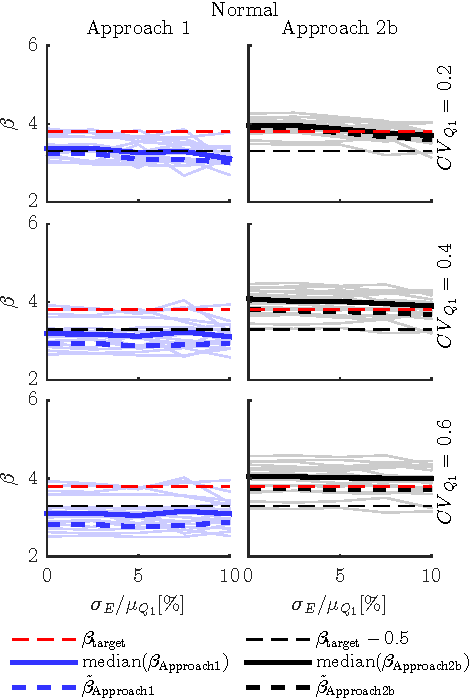
\includegraphics[]{Normal_additive_me_beta_smallm_666_median.pdf}
	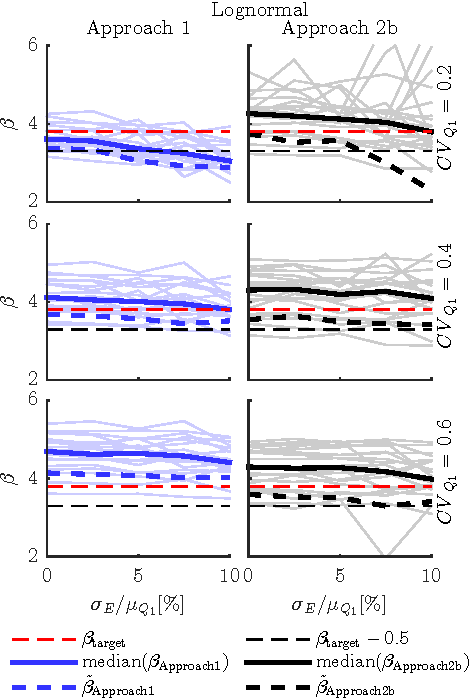
\includegraphics[]{Lognormal_additive_me_beta_smallm_666_median.pdf}
	\caption{Reliability indices as the function of the normalized standard deviation of measurement uncertainty ($\sigma_{E}/\mu_{Q_1}$). The thick solid lines are the median of the reliability indices while the thick dashed lines are the approximate predictive reliability indices.}
	\label{fig:Normal_lognormal_additive_me_beta_smallm}
\end{figure}

Comparing Approach~1 with Approach~2b for Normal and Gumbel distributions, the former approach yields to systematically lower reliability indices. The opposite trend observed for Lognormal distribution might be attributed to its heavy-tail. For Normal distribution, Approach~1 seems to be overly conservative, the median is well below the target reliability level. 
For all distributions, Approach~1 is reasonably conservative with the exception of Lognormal distribution and coefficient of variation of 0.6. However, even in this case the predictive reliability index corrects the overestimation. Though for Normal distribution it is too conservative, the currently prevalent Approach~1 appears to be safely applicable to measurement uncertainty problems in case of additive reality-observation relationship. Approach~2b is sound from theoretical point of view; however, its median overestimates reliability level, thus the predictive reliability index is to be used to avoid underestimation of failure probability. Its larger parameter estimation uncertainty can lead large reduction in reliability index for small sample sizes.
\begin{figure}[htbp!] 
	\centering    
	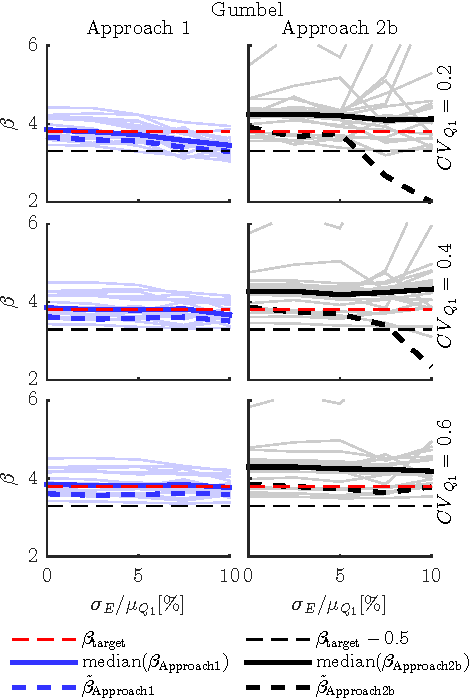
\includegraphics[]{Gumbel_additive_me_beta_smallm_666_median.pdf}
	\caption{Reliability indices as the function of the normalized standard deviation of measurement uncertainty ($\sigma_{E}/\mu_{Q_1}$). The thick solid lines are the median of the reliability indices while the thick dashed lines are the approximate predictive reliability indices.}
	\label{fig:Gumbel_additive_me_beta_smallm}
\end{figure}

%****************************************************************************************
%****************************************************************************************
\section{Application example: Turbine hall of Paks Nuclear Power Plant}
\label{sec:turbine_mu}

The turbine hall of Paks Nuclear Power Plant is selected to demonstrate the effect of measurement uncertainty on a real life example. The structure is introduced in Annex~\ref{sec:paks}, here only the essential details, which are required to interpret the results, are provided. The interval approach is used to represent measurement uncertainty and the two-step approximation is applied to propagate interval uncertainty. Annual ground snow maxima related to the location are contaminated with measurement uncertainty, the rest of random variables are represented by probability distributions. The results in terms of reliability indices and failure probabilities are given in Figure~\ref{fig:interval_beta_turbine_hall}. One year reference period is used for all calculations of the frame.

\begin{figure}[htbp!] 
	\centering    
	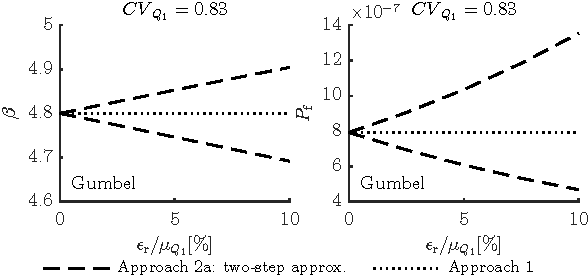
\includegraphics[]{interval_beta_turbine_hall.pdf}
	\caption{Reliability index and failure probability intervals as the function of normalized measurement uncertainty radius ($\epsilon_\mathrm{r}/\mu_{Q_1}$). Comparison of Approach~1 and Approach~2a for the turbine hall of Paks Nuclear Power Plant.}
	\label{fig:interval_beta_turbine_hall}
\end{figure}

The widest reliability index interval is 0.2, which is obtained for the largest measurement uncertainty error radius. This small value is in agreement with the trend observed in the previous example (Figure~\ref{fig:beta_interval_small_multiples}). It is attributed to the large coefficient of variation of annual ground snow load that is dominating over measurement uncertainty. In this example, neglect of measurement uncertainty leads to 70\% underestimation of failure probability at worst; hence, the effect is negligible.

%****************************************************************************************
%****************************************************************************************
\section{Discussion}
\label{sec:discussion_mu}
One can distinguish two components of measurement uncertainty: the reality-observation link and the nature of the contamination $E$. The three approaches considered here differ in how they treat these two components. The present prevalent approach (Approach~1) neglects both components, thus entirely ignores the possibility that the real values are greater or smaller than the observed due to measurement uncertainty.

The interval approach (Approach~2a) expresses full ignorance in respect of reality-observation link and represents measurement uncertainty with intervals. Therefore, no decoupling of true values from measurement uncertainty is possible. Intervals should be used with caution because by definition values outside of the interval are impossible. This assumption is rarely met in civil engineering. Measurement uncertainty is often described on the basis of expert judgment and wide intervals are applied to almost surely capture real, unobserved values.

The statistical approach (Approach~2b) requires the knowledge of the reality-observation link and represents measurement uncertainty with distribution function. This is the only approach that can decontaminate the observations and can directly infer the variable of interest, true variable. This is important since structural reliability is dependent on the true variable. The statistical and interval analysis based approaches are conceptually different, thus they are only comparable on that level but not quantitatively. Their uncertainty representation is inherently distinct, thus there is no equivalency between interval and distribution based representations.

Additionally, it must be emphasized that another type of uncertainty – statistical uncertainty in parameter estimation and selection of distribution function – often needs to be taken into account in reliability analysis as it may be even more important as measurement uncertainty investigated here \citep{RozsasIABSE2015, RozsasESREL2015}. Bayesian paradigm is a natural choice to incorporate this uncertainty, consequently that is recommended for practical applications. For example, in real-life situations, the reality-observation link cannot be established with certainty. Yet, this uncertainty can be captured by using multiple models and averaging them with respect their goodness of describing the data, this can be achieved for example by Bayesian model averaging \citep{Hoeting1999}.

Although this study is limited by the considered distribution types, reality-observation functions, and parameter range, it is believed to cover many practically relevant random variables. The presented approaches and algorithms can be easily used for other distribution types and measurement error structure. An additional limitation of this study is that measurement uncertainty is considered only for the dominant variable action. However, it is anticipated that for other random variables the effect is smaller due to their typically smaller sensitivity factor. Moreover, measurement uncertainty is much smaller for other than climatic actions such as resistance and permanent actions. Furthermore, the effect of sample size should be analyzed in later works. It is believed that the outcomes would be similar for sample sizes ranging from 20 to couple of hundreds, which cover the majority of cases in civil engineering. More data would allow more certain model identification.

%\section{Application example}

\section{Summary and conclusions}
The current practice in probabilistic engineering treats observed data contaminated with measurement uncertainty as realizations of the true distribution, thus neglecting the contamination mechanism. Statistical and interval-based analyses are thus conducted to investigate the effect of this simplification on structural reliability. Extensive parametric analyses -- based on 50 realizations, which is a typical length of records for climatic actions -- reveal that:\\
If interval representation of measurement uncertainty is used:
\begin{itemize}
	\item Sampling variability (parameter estimation uncertainty) has significant effect on reliability: it is dominant over measurement uncertainty for small interval radiuses and comparable for large radiuses.
	\item For mountains and highlands, moderate $\pm 4\%$ measurement uncertainty -- relative to value of an observed variable -- can lead to significant reduction of reliability level. For lowlands, even a large $\pm 10\%$ measurement uncertainty has no significant effect. An effect is deemed significant if it yields to greater than six fold increase in failure probability compared with Approach~1 (neglect of measurement uncertainty).
	\item Reliability interval ranges indicate that a small $\pm 2\%$ measurement uncertainty can lead to reduction of 0.6 in reliability index. For larger measurement uncertainties, the width of the reliability intervals can be larger than 2.0.
	\item The effect of measurement uncertainty is more pronounced for low variability random variables where its contribution to the total uncertainty increases.
	\item Parameter ranges where Approach~1 often overestimates the reliability index are identified.
\end{itemize}
If statistical (distribution function) representation of measurement uncertainty is used:
\begin{itemize}
	\item It is demonstrated that the statistical approach can be used to decontaminate the observations, thus to access the variable of interest.
	\item The ratio of the predictive and median failure probabilities can be as large as an order of magnitude or larger ($\sim30$ for Lognormal distribution).
	\item If parameter estimation uncertainty is disregarded, the reliability index can be considerably overestimated.
	\item For all considered distributions with additive measurement uncertainty, Approach~1 is reasonably conservative in most cases.
\end{itemize}

Practical recommendations:
\begin{itemize}
	\item Figure \ref{fig:beta_interval_small_multiples} and Figure \ref{fig:dspt_ratio_small_multiples} can be used to identify cases when Approach~1 significantly overestimates reliability index. In such cases and when no or very limited information on measurement uncertainty is available, then interval analysis could be used, considering the lower bound of the reliability interval.
	\item If the reality-observation link is known then the statistical approach is recommended. For small and moderate sample sizes ($<100$), the predictive reliability index is recommended. For additive measurement uncertainty, Approach~1 is conservative.
	\item For point estimates, such as median, the reliability index should be accompanied by uncertainty intervals to indicate the credibility of results.
	\item For ground snow extremes at lowlands, Approach~1 provides a reasonable approximation, thus the effect of measurement uncertainty can be neglected. Otherwise more advanced analysis is recommended.
\end{itemize}

Assessment of measurement uncertainty should be region- and case-specific accounting for measuring techniques, and applied correction equations, thus involvement of meteorologists, analysts or other experts is beneficial. Moreover, the selected approach to propagate measurement uncertainty should always be based on the particular issue in question, acknowledging ``the degree of precision to which the nature of the subject admits''.